\documentclass{zjureport}
% =============================================
% Part 1 Edit the info
% =============================================

\newcommand{\major}{信息工程}
\newcommand{\name}{徐阳}
\newcommand{\stuid}{3171002333}
\newcommand{\newdate}{2017-10-09}
\newcommand{\loc}{寝室}

\newcommand{\course}{数字信号处理}
\newcommand{\tutor}{Hao}
\newcommand{\grades}{59}
\newcommand{\newtitle}{系统传输函数零极点分析}
\newcommand{\exptype}{设计实验}
\newcommand{\group}{None}

% =============================================
% Part 1 Main document
% =============================================
\begin{document}
\thispagestyle{empty}
\begin{figure}[h]
  \begin{minipage}{0.6\linewidth}
    \centerline{
\includegraphics[width=\linewidth]{head.jpg}}
  \end{minipage}
  \hfill
  \begin{minipage}{.4\linewidth}
    \raggedleft
    \begin{tabular*}{.8\linewidth}{ll}
      专业: & \underline\major   \\
      姓名: & \underline\name    \\
      学号: & \underline\stuid   \\
      日期: & \underline\newdate \\
      地点: & \underline\loc
    \end{tabular*}
  \end{minipage}
\end{figure}

\begin{table}[!htbp]
  \centering
  \begin{tabular*}{\linewidth}{llllll}
    课程名称: & \underline\course   & 指导老师: & \underline\tutor   & 成绩:       &  \underline\grades \\
    实验名称: & \underline\newtitle & 实验类型: & \underline\exptype & 同组学生姓名:& \underline\group
  \end{tabular*}
\end{table}

% =============================================
% Part 2 Main document
% =============================================

\section{实验目的和要求}
  系统差分方程和传输函数是线性系统的重要概念,通过分析系统差分方程和传输函数的特性,编程查看系统零极点分布,加深对线性系统的了解。
\section{实验内容和步骤}

  \subsection{实验内容}

    给出如下差分方程:
    $$y(n) - (0.5+a)\times y(n-1) + 0.5ay(n-2) = x(n)$$
    \begin{clause}
      \item 求解系统传输函数表达式。
      \item 当a取0.8,0.9,1.0,1.1时,画出零极点分布图。
      \item 根据(2)中a的取值,分别画出幅频响应函数。
    \end{clause}

  \subsection{实验步骤}
    \begin{clause}
      \item 编写程序,求解零极点
      \item 画出图形。
      \item 观察结果。
    \end{clause}

\section{主要仪器设备}
  计算机,Matlab软件

\section{操作方法和实验步骤}
  \subsection{传输函数}
    对差分方程进行处理,求出传输函数表达式。
  \subsection{零极点分布图}
    在此基础上,使用Matlab中的zplane函数进一步画出在不同a取值情况下的零极点分布图。
  \subsection{幅频响应}
    之后使用freqz函数画出不同a取值情况下的频率响应图像。

\section{实验数据记录和处理}
  \subsection{传输函数}
    根据差分方程,传输函数如下:
    $$H(z) = \frac{Y(z)}{X(z)} = \frac{z^2}{z^2-(0.5+a)z+0.5a}$$
  \subsection{零极点分布图}
    a = 0.8,0.9,1.1时,系统的零极点分布图及程序如下:
    \begin{clause}
      \item 图像
      \begin{center}
        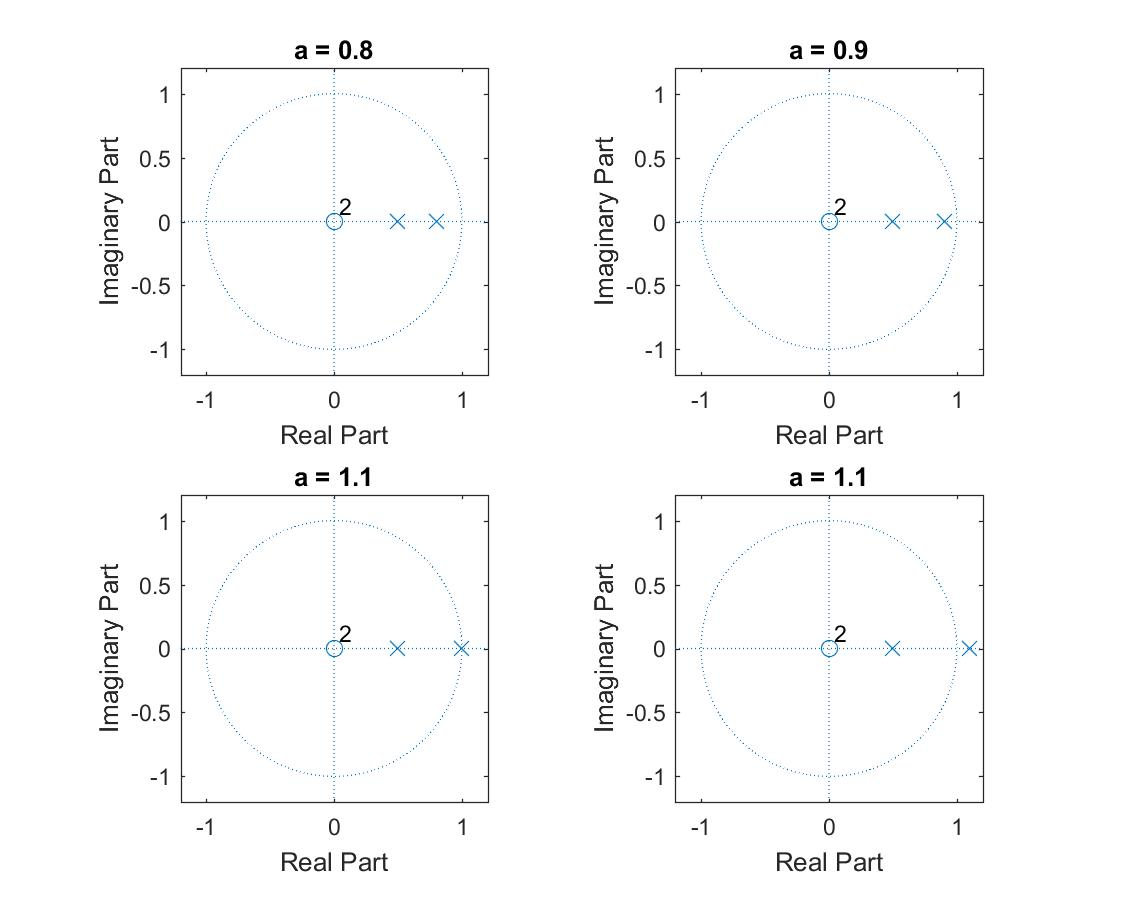
\includegraphics[width=0.6\linewidth]{01.jpg}
      \end{center}
      \item 代码
      \lstinputlisting[language=MATLAB]{code/do.m}
    \end{clause}

  \subsection{频率响应}
    a = 0.8,0.9,1.0,1.1时,系统的频率响应函数图形及程序如下:
    \begin{clause}
      \item 图像
      \begin{center}
        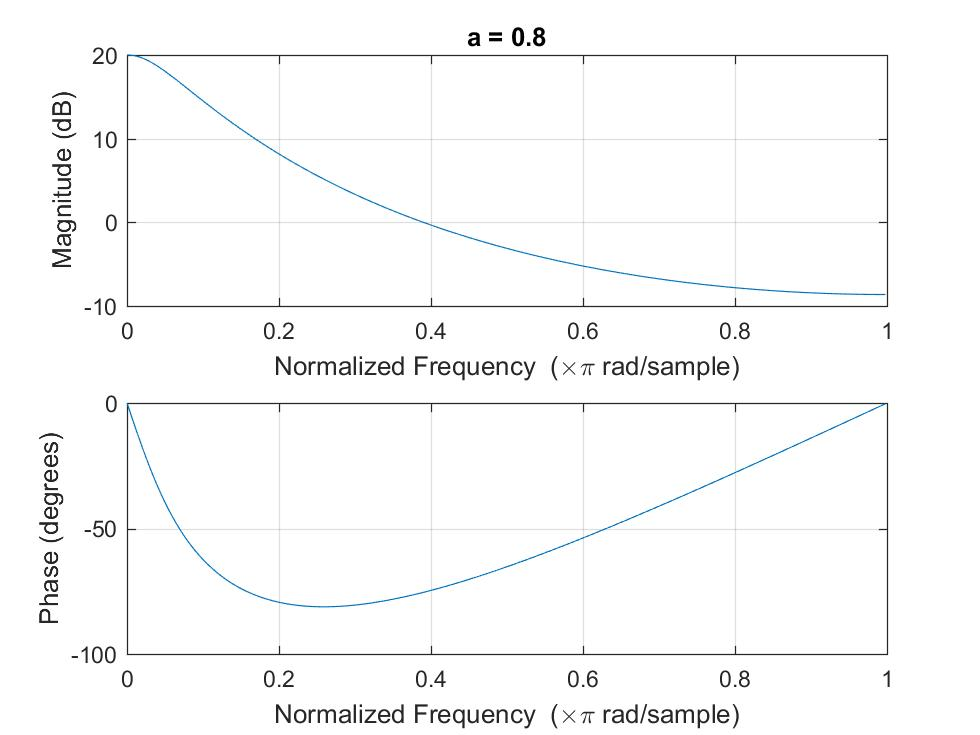
\includegraphics[width=0.6\linewidth]{02-1.jpg}
      \end{center}
      \item 代码
      \lstinputlisting[language=MATLAB]{code/next.m}
    \end{clause}

\section{实验结果与分析}

balabalabala

\end{document}
